\textbf{\underline{OZ 6 - Magnetische inductie en de wet van Faraday - Oefening 1:}}
\vspace{0.5cm}

    \vspace{-0.5cm}\begin{minipage}{.8\textwidth}
        Een kort stuk van een draad, van lengte $a$, beweegt met snelheid $\vec{v}$ , parallel langs
        een zeer lange draad waardoor een stroom $I$ loopt d. Het dichtste uiteinde
        van de korte draad is een afstand b van de lange draad verwijderd. Neem aan dat de
        verticale draad lang is vergeleken met a + b. Bepaal de emf tussen de uiteindes van
        de korte draad wanneer $\vec{v}$ (a) in de zelfde zin is als I, en (b) in de tegengestelde zin
        is als $I$.
    \end{minipage}
    \hspace{0.5cm}\begin{minipage}{.16\textwidth}
        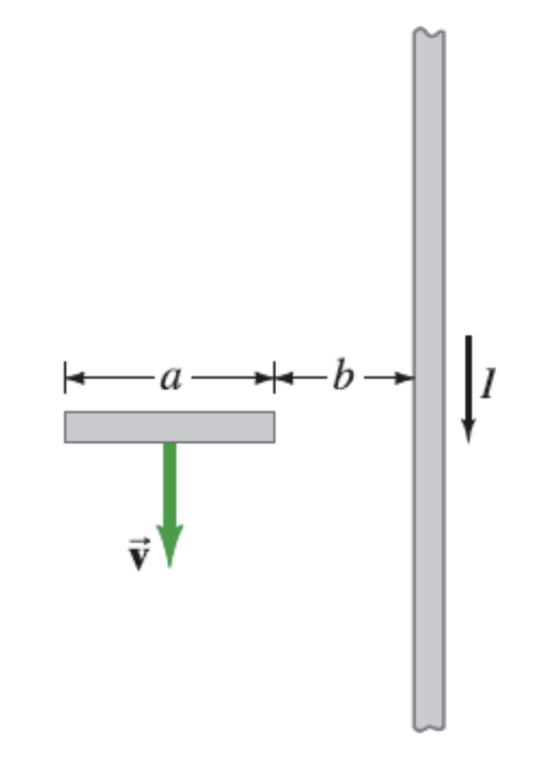
\includegraphics[scale = 0.25]{oz06/resources/Oz6Oef1.png}
    \end{minipage}

    \begin{description}[labelwidth=1.5cm, leftmargin=!]
        \item[Geg. :]
        \item[Gevr. :] 
        \item[Opl. :]
    \end{description}


\vspace{1cm}